\documentclass[11pt,a4paper]{article}
\usepackage[top=3cm, bottom=2cm, left=3cm, right=2cm]{geometry}
\usepackage[utf8]{inputenc}
% \usepackage[T1]{fontenc}
\usepackage{amsmath, amsfonts, amssymb}
\usepackage{siunitx}
\usepackage[brazil]{babel}
\usepackage{graphicx}
\usepackage[margin=10pt,font={small, it},labelfont=bf, textfont=it]{caption}
\usepackage[dvipsnames, svgnames]{xcolor}
\DeclareCaptionFont{MediumOrchid}{\color[svgnames]{MediumOrchid}}
\usepackage[pdftex]{hyperref}
\usepackage{natbib}
\bibliographystyle{plainnat}
\bibpunct{[}{]}{,}{s}{}{}
\usepackage{color}
\usepackage{footnote}
\usepackage{setspace}
\usepackage{booktabs}
\usepackage{multirow}
\usepackage{subfigure}
\usepackage{fancyhdr}
\usepackage{leading}
\usepackage{indentfirst}
\usepackage{wrapfig}
\usepackage{mdframed}
\usepackage{etoolbox}
\usepackage[version=4]{mhchem}
\usepackage{enumitem}

\setlist[itemize]{label=\textcolor{CarnationPink}{$\mathbf{\square}$}}

\setlist[enumerate]{label=\textcolor{CarnationPink}{\arabic*.}, align=left}


\newcounter{exemplo}

\NewDocumentEnvironment{exemplo}{ O{} }{%
\allowbreak
\setlength{\parindent}{0pt}
  \begin{mdframed}[
  leftline=true,
  topline=false,
  rightline=false,
  bottomline=false,
  linewidth=2pt,
  linecolor=CarnationPink,
  frametitlerule=false,
  frametitlefont=\Large\bfseries\color{CarnationPink},
  frametitle={\color{CarnationPink}\normalfont\bfseries #1},
  ]
}{%
  \end{mdframed}
}

\setlength{\fboxsep}{10pt}
\setlength{\fboxrule}{1pt}
\usepackage{float}
\renewcommand{\thefootnote}{\alph{footnote}}
\usepackage{url}
\hypersetup{
    colorlinks=true,
    linkcolor=cyan,
    filecolor=cyan,      
    urlcolor=cyan,
    citecolor=cyan,
    pdftitle={Resumos}
}
\pagestyle{fancy}
\fancyhf{}
\renewcommand{\headrulewidth}{0pt}
\rfoot{Página \thepage}

\title{Resumo}
\author{Radiações Ionizantes e Dose Absorvida \nocite{*}}
\date{\textit{Dalila Mendonça}}
\begin{document}
	\maketitle

\begin{exemplo}[3. Radiação Ionizante]
    \textcolor{CarnationPink}{Interação de Fótons}
    \begin{itemize}
        \item Os cinco principais tipos de interações de fótons com a matéria em ordem de limiar de energia são (1) espalhamento de Rayleigh, também conhecido como espalhamento coerente, espalhamento clássico ou espalhamento elástico; (2) efeito fotoelétrico, também conhecido como absorção fotoelétrica; (3) espalhamento Compton, também conhecido como espalhamento incoerente, ou efeito Compton; (4) produção de pares; e (5) fotodesintegração nuclear ou Efeito fotonuclear.
        
        \item No espalhamento Rayleigh, o fóton incidente interage com o átomo como um todo, espalhando-se em uma direção diferente sem perder energia. Não ocorre ionização no espalhamento Rayleigh porque os elétrons não são ejetados.
        
        \item No efeito fotoelétrico, toda a energia do fóton incidente é transferida para um elétron orbital, que é então ejetado do átomo. A energia do elétron ejetado (fotoelétron) é a energia do fóton incidente menos a energia de ligação. A emissão de raios-X característicos ou elétrons Auger ocorrerá subsequentemente, preenchendo a lacuna do fotoelétron.
        
        \item O espalhamento Compton é uma colisão entre um fóton e um elétron orbital de camada externa fracamente ligado de um átomo, resultando em um fóton espalhado de menor energia e um elétron com determinada energia cinética. Esta é a interação dominante dos feixes de raios X terapêuticos com o tecido. Como a energia do fóton incidente excede em muito a energia de ligação do elétron da camada externa, a interação Compton parece uma colisão entre o fóton e um elétron livre (denominado quase livre).
        
        \item Na produção de pares, o fóton interage fortemente com o campo eletromagnético de um núcleo atômico e perde toda a sua energia para criar um elétron e um pósitron.
        
        \item Na fotodesintegração, um fóton incidente com alta energia (>7 a 10 MeV) colide com o núcleo de um átomo e toda a energia do fóton é absorvida. O núcleo então emite um nêutron. Este efeito causa requisitos extras de blindagem para feixes de alta energia.
        
        \item Com um fóton de entrada, as partículas de saída produzidas pelas quatro interações de fótons são listadas a seguir:
            \begin{enumerate}[label=\roman*.]
                \item Espalhamento Rayleigh: um fóton;
                \item Efeito fotoelétrico: um elétron;
                \item Espalhamento Compton: um elétron e um fóton;
                \item Produção de pares: um elétron e um pósitron.
            \end{enumerate}

        \item O efeito fotoelétrico é proporcional a $Z^3/E^3$, onde Z é o número atômico do átomo alvo e E é a energia do fóton incidente.
        
        \item A probabilidade de espalhamento Compton é independente de Z e diminui com E. O espalhamento Compton depende da densidade eletrônica$N_e$ do material.
        
        \item A probabilidade de produção de pares muda com $Z^2$ e log(E).
        
        \item O espalhamento Compton é mais provável de ocorrer com os elétrons da camada externa.
        
        \item A energia mínima de um fóton incidente para o processo de produção de pares é de 1,02 MeV. Essa energia corresponde à massa do elétron e do pósitron produzidos (0,511 MeV cada). A energia adicional acima do limite de 1,02 MeV é convertida em energia cinética para o par.
        
        \item O efeito fotoelétrico é a principal causa da absorção dos fótons com energia de 10 a 100 keV em água. Esta é a faixa dos raios-X de diagnóstico. A dependência da absorção do número atômico $Z^3$ fornece o excelente contraste das imagens de raios-x diagnósticas.
        
        \item O espalhamento Compton é a principal causa da absorção de fótons com energia de 100 keV–10 MeV na água. Esta é a faixa dos raios-X terapêuticos.
        
        \item O efeito fotoelétrico é mais provável quando a energia do fóton é ligeiramente maior que a energia de ligação do elétron orbital. No espectro de absorção, as energias de ligação das camadas aparecem como picos agudos conhecidos como “bordas de absorção”, rotulados pela camada correspondente, por exemplo, borda K, para absorção da camada mais interna.
        
        \item KERMA é a Energia Cinética Liberada por unidade de MAss e representa a energia transferida para o meio pelo fóton.
        
        \item As probabilidades de espalhamento Compton e efeito fotoelétrico são aproximadamente as mesmas para fótons de aproximadamente 30 keV interagindo com tecidos moles.
        
        \item No espalhamento Compton, à medida que a energia do fóton incidente aumenta, tanto os fótons quanto os elétrons são espalhados mais na direção direta. Além disso, a proporção de energia transportada pelo elétron espalhado aumenta com a energia do fóton incidente.
        
        \item No espalhamento Compton, a energia máxima do fóton espalhado é 511 keV a 90° e 255 keV a 180° (ou seja, retroespalhamento). Estas são as energias de interesse para blindagem secundária.
        
        \item Uma vacância criada na camada K causa a transição de um elétron de uma camada superior para a camada K. Isso pode criar uma vacância na camada intermediária (por exemplo, L ou M) que pode ser preenchida por um elétron de camada ainda mais alta. Essa cascata de elétrons continua à medida que os elétrons da camada externa saltam para as camadas internas. A diferença em suas energias de ligação é liberada como raios-X característicos ou elétrons Auger.
    \end{itemize}

    \textcolor{CarnationPink}{Interação de Partículas}
    \begin{itemize}
        \item Partículas alfa (\ce{\alpha2+} ou \ce{He2+}), prótons (p+), partículas beta (\ce{\beta-}), pósitrons (\ce{\beta+}) e elétrons (e-) são alguns exemplos de partículas carregadas. Fótons (ou seja, raios X e raios gama), nêutrons e neutrinos são alguns exemplos de partículas sem carga.
        
        \item As partículas carregadas podem sofrer três tipos de interação: excitação, ionização e produção bremsstrahlung. Excitação e ionização são interações da partícula carregada com os elétrons orbitais. Bremsstrahlung é uma interação da partícula carregada com o núcleo.
        
        \item A principal diferença entre excitação e ionização está relacionada ao elétron orbital ser ou não ser ejetado do átomo. Na excitação, a energia transferida não excede a energia de ligação do elétron, então o elétron é elevado a um nível de energia mais alto mas ainda se mantém ligado ao átomo. Na ionização, a energia transferida excede a energia de ligação do elétron, então o elétron é ejetado do átomo.
        
        \item Raios X, raios gama, elétrons, prótons, partículas alfa e nêutrons são alguns exemplos de radiação ionizante. Microondas, ondas de rádio e fótons ópticos são alguns exemplos de radiação não ionizante.
        
        \item A radiação diretamente ionizante vem de partículas carregadas (por exemplo, prótons, elétrons e partículas alfa) e a radiação indiretamente ionizante vem de partículas não carregadas (por exemplo, fótons e nêutrons).
        
        \item Os raios delta são elétrons secundários com energia suficiente para percorrer uma distância significativa do feixe de radiação primário e produzir mais ionização (ou seja, ionização secundária).
        
        \item O número médio de pares de íons primários e secundários produzidos por unidade de comprimento do caminho da partícula carregada é chamado de Ionização Específica (IS). O SI geralmente é expresso em unidades de pares de íons por mm (par de ions/mm).
        
        \item A  Ionização Específica aumenta com $Q^2$ e diminui com $v^2$. Assim, $IS \propto Q^2/v^2$.
        
        \item À medida que um próton viaja através da matéria, ela perde velocidade, fazendo com que sua ionização específica (IS) aumente até um máximo, chamado de pico de Bragg, quando ela para definitivamente. A ionização específica cai rapidamente depois que o próton deposita sua energia.
        
        \item O comprimento do caminho de uma partícula é a distância que a partícula percorre, enquanto o alcance de uma partícula é a profundidade de penetração da partícula na matéria. O comprimento do caminho percorrido de um elétron individual quase sempre excede seu alcance, enquanto o comprimento do caminho percorrido de uma partícula carregada pesada (por exemplo, partículas alfa) é essencialmente igual ao seu alcance.
        
        \item A LET é a quantidade média de energia depositada localmente na matéria por unidade de comprimento do caminho. A LET é frequentemente expressa em unidades de keV por \unit{\mu m} (\unit{keV/\mu m}).
        
        \item O LET de uma partícula carregada aumenta com $Q^2$ e diminui com $E_k$. Assim, $LET \propto Q^2/E_k$
        
        \item Partículas alfa, prótons e nêutrons são exemplos de radiação com alta LET. Elétrons, raios X e raios gama são exemplos de radiações de baixa LET.
        
        \item À medida que um elétron interage com um núcleo atômico, ele é desviado de sua trajetória e desacelerado pelo núcleo carregado positivamente, com perda de energia cinética que leva a emissão de raios-X bremsstrahlung. Bremsstrahlung é uma palavra alemã que significa ``radiação de freamento''.
        
        \item A emissão total de bremsstrahlung por átomo aumenta com $Z^2$ e diminui com $m^2$. Assim, bremsstrahlung $\propto Z^2/m^2$.
        
        \item Um pósitron interage com um elétron no final de seu alcance, resultando na aniquilação do par elétron-pósitron e na conversão de sua massa de repouso em energia na forma de dois fótons de 0,511 MeV com direções opostas.
        
        \item O poder de freamento de uma partícula carregada é a perda de energia por unidade de comprimento de caminho em um meio, geralmente dado em unidades de MeV/m ou joule (J/m).
        
        \item O poder de freamento mássico de uma partícula carregada é o poder de freamento dividido pela densidade do meio, geralmente dado em unidades de MeV m2/kg ou J m2/kg.
        
        \item De acordo com o destino da energia perdida pela partícula carregada, o poder de freamento pode ser dividido em “poder de freamento de colisão”, resultado da excitação e ionização e “poder de freamento radiativa”, resultado da produção bremsstrahlung.
        
        \item Analisando a velocidade relativa das partículas alfa, prótons e elétrons com a mesma energia cinética, a velocidade da partícula $\alpha^{2+} < p^{+} < e^{-}$. A energia cinética depende da massa e do quadrado da velocidade. Para a mesma energia, a partícula mais leve será a mais rápida, então a classificação segue a massa das partículas.
        
        \item Analisando o alcance relativo das partículas alfa, prótons e elétrons com a mesma energia cinética, o alcance da partícula $\alpha^{2+} < p^{+} < e^{-}$. O alcance é proporcional à massa e inversamente proporcional ao quadrado da carga elétrica.
        
        \item Os feixes prótons e as partículas carregadas pesadas usados em tratamentos permitem concentrar a dose dentro do tumor enquanto as doses no tecido sadio aos arredores do tumor é minimizada. Isto ocorre devido às caracteristicas de interação destas partículas. A medida que as partículas carregadas são desaceleradas, elas liberam mais energia no meio, e esta propriedade causa o pico de bragg, caracterizado como uma grande deposição de energia no final do alcance da partícula. 
        
        \item Os dois principais tipos de interações de nêutrons com a matéria são o espalhamento e a absorção. Os nêutrons podem interagir com os núcleos por meio de espalhamento em colisões semelhantes a “bolas de bilhar”, produzindo núcleos de recuo que depositam sua energia por meio de excitação e ionização. Os nêutrons também podem ser absorvidos por núcleos e causar uma variedade de emissões, como raios gama, partículas carregadas, nêutrons ou fragmentos de fissão.
        
        \item Os nêutrons não causam excitação e ionização diretamente. Como os nêutrons são partículas sem carga eles não interagem com os elétrons via excitação e ionização.
        
        \item O efeito Cerenkov ocorre quando uma partícula carregada viaja em um meio a uma velocidade maior que a velocidade da luz nesse meio (nenhuma partícula massiva pode viajar mais rápido que a luz no vácuo). Nessa condição, a partícula carregada cria uma “onda de choque” eletromagnética, semelhante à onda de choque acústica quando um avião viaja mais rápido que a velocidade do som. A onda de choque eletromagnético aparece como uma explosão de radiação visível, conhecida como radiação de Cerenkov. Potencialmente, isso poderia ser usado para medir a posição e a intensidade da dose depositada. A probabilidade de ocorrência do efeito Cerenkov é muito pequena (muito menos de 1\%), mas alguns pacientes que recebem tratamento com elétrons perto dos olhos podem descrever a visão de anéis azulados durante o tratamento.
        
    \end{itemize}
\end{exemplo}


\begin{exemplo}[4. Dose Absorvida]

    \textcolor{CarnationPink}{Dosimetria}
    \begin{itemize}
        \item A exposição é definida como o quociente $dQ/dm$, onde dQ é a carga total de íons de um sinal que são produzidos no ar quando todas as partículas carregadas produzidas por fótons são completamente freadas, e dm é a massa de ar dentro da qual as partículas carregadas são liberadas. 
        
        \item A definição de exposição requer que as partículas carregadas sejam completamente paradas no ar. Para feixes de megavoltagem, o alcance de partículas carregadas no ar é muito grande para que a medição da exposição seja possível.
        
        \item O roetgen( R) é a unidade de exposição. A unidade original foi definida como a quantidade de radiação que libera 1 esu (unidade eletrostática) de carga por centímetro cúbico de ar. Para expressar o roentgen em unidades SI, usamos o fator de conversão de esu para C (Coulombs) e a densidade do ar (aproximadamente 1,293 \unit{kg/m^3}). Como 1 esu  \qty{3.34e{-10}}{C}, temos
        
        $$1R = 1 \frac{esu}{cm^3} = \frac{1\;esu \times 3.34 \times 10^{-10} \frac{C}{esu}}{1\;cm^3 \times 1.293 \frac{kg}{m^3} \times \frac{m^3}{10^6 cm^3}} = 2.58 \times 10^{-4} \frac{C}{kg}$$

        \item O fator $f$ é usado para converter a exposição, que é definida apenas no ar, para a dose em um meio. É denominado o fator roentgen para rad. Para o ar, f é 0,876.
        
        \item Assumindo que o equilíbrio de partículas carregadas existe no ponto de interesse, a dose em um meio pode ser calculada a partir da exposição a partir da seguinte equação:
        
            $$D_m(cGy) = f \times X \times \frac{\Psi_m}{\Psi_{ar}}$$

        onde X é a exposição (R) e $\Psi_{m}/\Psi_{ar}$ é a razão da fluência de energia de um meio m com o ar. O fator $f$ para a agua varia de 0.88 até 0.97 dependendo da energia dos raios X.


        \item O fator $f$ é definido como:
        
            $$f = 0.876 \frac{\left(\frac{\bar{\mu}_{ab}}{\rho}\right)_m}{\left(\frac{\bar{\mu}_{ab}}{\rho}\right)_{ar}}$$

        O numerador contém o coeficiente mássico de absorção de energia para o material de interesse enquanto que o denominador contém o coeficiente mássico de absorção de energia para o ar. Diferentes materiais possuem diferentes seções de choque para as interações e portanto $f$ é inerentemente dependente do meio. O coeficiente mássico de absorção de energia também é dependente da energia do feixe incidente uma vez que diferentes processos de interação são dominantes para diferentes energias. 

        \item A dose absorvida é a energia absorvida por unidade de massa. Esta é uma quantidade física mensurável. A unidade de medida padrão para a dose absorvida é o gray (Gy), no qual é definida como 1 joule de energia absorvida por 1 kg de massa.
        
        \item A dose absorvida é um dos fatores utilizados para explicar o efeito biológico causado pela radiação no tecido. No entanto, o efeito biológico causado pela radiação também depende de outros fatores relacionados à radiação como o tipo de radiação e a taxa com o qual a radiação é entregue.
        
        \item Ao utilizar uma câmara de ionização para mensurar a dose absorvida, utiliza-se a teroria cavitária de Bragg-Gray que permite relacionar o número de ions coletados na câmara com a dose absorvida no meio no qual a câmara está inserida. 
        
        \item Segundo a teoria cavitária de Bragg-Gray, a dose absorbida no meio ao redor da câmara está relacionada com a dose no ar dentro da câmara através da razão da média dos poderes de freamento mássico do meio e do gás dentro da câmara, no qual será equivalente à razão entre a dose no meio e a dose no gás.
        
        \item Para uitilizar a teoria cavitária de Bragg-Gray para determinar a dose abvsorvida no meio através da dose em uma cavidade inserida nesse meio deve-se assumir que: Primeiro, a presença do meio da cavidade não afeta o campo de partículas carregadas porque sua espessura é pequena em comparação com o alcance de partículas carregadas que incidem sobre ele. Em segundo lugar, toda a dose no meio da cavidade é depositada pelas partículas carregadas que o atravessam.
        
        \item A difefença entre a teoria cavitária de Bragg-Gray e a Teoria cavitária de Spencer Attix é que a teoria cavitária de Spencer-Attix utiliza o poder de freamento mássico restrito com um valor de corte de $\Delta$ (normalmente 10–20 keV) para levar em consideração o efeito dos raios delta que depositam apenas parte de sua energia no volume de interesse e pode depositar energia em uma distancia além do volume em questão. Spencer-Attix é, portanto, mais preciso que Bragg-Gray.
        
        \item O Equilíbrio de Paartículas Carregadas é o conceito de que dado um volume $V$, cada partícula carregada de um sinal e energia saindo de $V$ é, em média, substituída por uma partícula carregada idêntica da mesma energia entrando em $V$.
        
        \item De acordo com o TG-51, a equação para calibração dos aceleradores lineares é:
        
            $$D_W^Q = N_{D,w}^{{}^{60}Co} M k_Q$$
        
        onde $D_W^Q $ é a dose absorvida na água medida no ponto de referência em um feixe de qualidade $Q$ (Sua unidade é Gy). $N_{D,w}^{{}^{60}Co}$ é o coeficiente de calibração para conversão da carga medida para a dose (Sua unidade é Gy/C). $M$ é a leitura do eletrômetro corrigida, em unidades de C. $k_Q$ é o fator de correção para a qualidade no qual corrige o coeficiente de calibração devido as diferenças nas qualidades do feixe entre o feixe que está sendo calibrado e o feixe de \ce{^{60}Co}.

        \item O fator de correção para temperatura e pressão dado no TG-51 é:
        
            $$k_{T,P} = \frac{760}{P} \times \frac{273.2 + T}{295.2}$$

        onde P é a pressão atmosférica em unidades de mmHg. Para P dado em unidades de kPa o fator de correção 1kPa = 7.5 mmHg deve ser utilizado. A Temperatura T dada em \unit{\celsius} é convertida para kelvin (K) adicionando 273.2; E 295.2 é a temperatura em kelvin sob as condições de referência.


        \item Para câmaras de ionização não seladas, a sua resposta pode mudar devido à variações na temperatura e pressão justamente porque a massa de ar dentro da câmara varia com a pressão e a temperatura. O fator $k_{T,P}$ corrige os desvios de temperatura e pressão das condições de referência (295,2 K e 760 mmHg) sob as quais a câmara foi calibrada.
        
        \item O protocolo TG-51 fornece um meio para calibrar a saída de um acelerador linear. O resultado é a calibração da dose em função das Unidades Monitoras (Mu's) em um ponto específico em um fantoma de água, a uma distância padrão, para um tamanho de campo de referência.
        
        \item Normalmente, a geometria de calibração é um tamanho de campo de referência de 10 cm x 10 cm, distância da fonte até a superfície da água de 100 cm e na profundidade nominal máxima da energia calibrada. A determinação da dose em outros pontos pode então ser calculada com base em fatores de saída medidos, por exemplo, razão de tecido máximo (TMR), fator de espalhamento do colimador (Sc), fator de espalhamento do phantom (Sp), razão off-axis (OAR), porcentagem de dose na profundidade (PDP), e assim por diante.
        
        \item A carga medida pelo eletrômetro depende da polaridade aplicada à câmara de ionização. Os fótons interagem não apenas com o gás na câmara de ionização, mas também com o eletrodo coletor central, ejetando elétrons no qual podem aumentar ou diminuir dependendo da polaridade aplicada à câmara de ionização. Uma corrente adicional fora da cavidade de coleta, conhecida como corrente extracameral, também pode ocorrer devido a circuitos mal blindados ou interações que ocorrem no cabo da câmara de íonização.
        
        \item A alta voltagem de uma câmara de ionização é usada para separar e coletar os íons que se formam na presença da radiação ionizante. O processo de coleta não é 100\% eficiente e alguns íons formados se recombinam antes de chegar aos eletrodos coletores, causando perda de sinal (uma vez recombinados, formam átomos com carga elétrica neutra, o qual não é acelerado pelo campo elétrico formado pela diferença de potencial aplicada na câmara).
        
        \item O fator de correção do eletrômetro, P\textsubscript{elec}, é necessário quando a câmara deionização e o eletrômetro não são calibrados como uma unidade (juntos). Este fator é fornecido por um Laboratório de Calibração de Dosimetria Credenciado (ADCL) e deve ser verificado novamente pelo ADCL a cada dois anos.
        
        \item Suponha que 1 g de água, 1 g de ar e 1 g de poliestireno absorvem cada um 1 J de energia, como a dose absorvida é definida como a energia absorvida por unidade de massa. Como cada meio absorveu a mesma quantidade de energia e também contém a mesma massa, todos recebem a mesma dose.
        
        \item Comparando um feixe de 10 MV de fótons e um feixe de 10 MeV de elétrons, a dose na pele para o feixe de elétrons é maior do que a dose para o feixe de fótons. Feixes de fótons de alta energia (>1 MV) são indiretamente ionizantes e, portanto, depositam sua dose downstream, em alguns centímetros de profundidade. Os feixes de elétrons, no entanto, são diretamente ionizantes. Os elétrons em um feixe de elétrons podem depositar uma dose significativa diretamente na superfície do paciente.
        
        \item A absorção de fótons é baseada na densidade eletrônica e no número atômico do meio. Um phantom água-equivalente deve ter a mesma densidade eletrônica (número de elétrons por \unit{cm^3} =  $3.34 \times 10^{23}$ para a água) e número atômico efetivo, Z\textsubscript{eff} = 7.42.
        
        \item KERMA é um acrônimo que significa “kinetic energy released per unit mass” “energia cinética liberada por unidade de massa”. É definido como a razão
        
            $$KERMA = \frac{dE_{tr}}{dm}$$

        onde $dE_{tr}$ é a energia cinética inicial total de todas as partículas carregadas colocadas em movimento pelos fótons em uma massa $dm$ do material. o Kerma também pode ser calculado através da equação:

            $$KERMA = \Psi \left(\frac{\bar{\mu}_{tr}}{\rho}\right)$$

        onde $\bar{\mu}_{tr}/\rho$ é coeficiente mássico médio de transferência de energia e $\Psi$ é a fluência de energia do fóton. O Kerma é expresso em unidades de J/kg. O KERMA pode ser dividido em componente de colisão (dose depositada) e radiativa (bremsstrahlung).
    \end{itemize}

    \textcolor{CarnationPink}{Dosímetros}
    \begin{itemize}
        \item Um dosímetro ideal deve ser capaz de medir a dose de radiação com precisão, com a mesma sensibilidade, independentemente do tipo de radiação, energia da radiação, taxa de dose ou histórico de exposição do dosímetro.
        
        \item Um dosímetro absoluto é aquele que não precisa ser calibrado antes de ser utilizado para medir a dose absoluta. Existem três tipos comuns de dosímetros absolutos: câmaras de ionização de ar livre, dosímetros Fricke de sulfato ferroso  e calorímetros.
        
        \item As câmaras de ionização de ar livre são grandes câmaras de ionização projetadas para medir a exposição. Seu grande tamanho e limitações de energia limitam principalmente seu uso a laboratórios de padrões nacionais.
        

        \begin{center}
            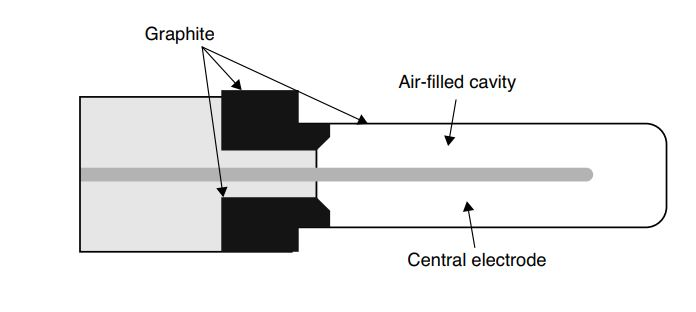
\includegraphics[width=0.4\textwidth]{Imagens/camaraDeIonização.JPG}
        \end{center}
        
        \item Uma câmara de ionização é composta por dois polos condutores e um espaço entre os polos preenchido com ar, A Radiação ioniza as moléculas de ar e forma um par elétron-íon (elétron com carga negativa e o íon com carga positiva). Essas partículas são conduzidas através de uma tensão de polarização para os dois polos da câmara e são coletadas pelo eletrômetro. O número de pares de ions produzidos e então a carga coletada nos polos é proporcional a dose de radiação recebida. A câmara de ionização é o tipo de dosímetro mais robusto para medir a dose absoluta e sua resposta é estável com respeito a taxa de dose, ou seja, a dose entregue é a mesma para a quantidade de MU entregue à diferentes taxas de dose.
        
        \item A voltagem de polarização em uma câmara de ionização é escolhida de forma que os pares de ions produzidos pela ionização direta se movam rápido o suficiente em direção aos polos de modo que não exista uma recombinação iônica significante, e ao mesmo tempo, a voltagem de polarização deve ser pequena o suficiente para que os pares de ions formados não tenham capacidade de causar mais ionizações, fazendo com que pares de ions extras sejam formados.  Normalmente é utilizada uma voltagem de polarização variando entre 150 V e 300 V (positivo ou negativo).
        
        \item A espessura da parede de uma câmara de ionização deve ser maior ou igual ao alcance das partículas secundárias carregadas (elétrons) que são produzidos na parede. Essa condição é necessária para fornecer o equilibrio eletrônico dentro do volume sensível da câmara. Em feixes de alta energia, esta condição não é satisfeita e uma capa de buil-up é necessária para fornecer uma espessura adicional à parede da câmara para manter a condição de equilíbrio eletrônico.
        
        \item A cavidade de uma câmara de ionização pode ser selada ou aberta para a atmosfera. A quantidade de ar dentro de uma câmara aberta depende da temperatura e pressão atmosférica no ponto de medida e portanto quando for realizada a medida da dose, a leitura de carga deve ser corrigida pela temperatura e pressão. Câmaras seladas fornecem uma resposta constante e não são afetadas por mudanças externas de temperatura e pressão, porém estas câmaras são vulneráveis à vazamentos.
        
        \item Uma câmara de ionização de placas paralelas também possui um volume sensível cilindrico, mas sua altura é muito menor que seu raio. Isto permite que a câmara realize medidas de um grande volume mas em uma pequena profundidade. Elas são comumente usadas para medir a dose perto da superfície de um fantoma ou na região de buil-up, além de serem utilizadas em medidas de feixes de elétrons que apresentam mudanças bruscas de dose em função da profundidade.
        
        \item As câmaras de extrapolação foram inicialmente projetadas para dosimetria de elétrons. Como câmaras de ionização têm extensão espacial finita, torna-se difícil sua utilização para medir a dose nas camadas superficiais de um meio (por exemplo, dose na superfície). As câmaras de ionização de extrapolação contêm parafusos micrométricos que são usados para ajustar o espaçamento entre seus eletrodos. A dose em um espaçamento de 0 cm pode ser extrapolada a partir de uma série de medições feitas em espaçamentos progressivamente menores. 
        
        \item Um Dosímetro Termoluminescente (TLD) é feito de materiais semicondutores que, quando expostos à radiação ionizante, permitem que os elétrons fiquem presos em estados metaestáveis (armadilhas). Quando aquecidos, esses elétrons caem no estado fundamental e a luz é liberada. A quantidade de luz liberada pelo material é então proporcional à dose de radiação. Após o aquecimento, o TLD pode ser reutilizado.
        
        \item Os materiais mais comuns utilizados na fabricação de dosímetros TLD são: 
        
            \begin{itemize}[label=\textopenbullet]
                \item \ce{LiF}:\ce{Mg},\ce{Ti}
                \item \ce{LiF}:\ce{Mg},\ce{Cu},\ce{P}
                \item \ce{Li2B4O7}:\ce{Mn}
                \item \ce{CaSO4}:\ce{Dy}
                \item \ce{CaSO4}:\ce{Mn}
            \end{itemize}
                
        \item O \ce{LiF}:\ce{Mg} é o tipo mais comum de dosímetros TLD e está disponível em várias formas incluindo pó, cartões, fitas e chips de Teflon. Este material possui uma densidade física de \qty{2.64}{g/cm^3} e número atômico efetivo $\mathrm{Z_{eff} = 8.2}$, que é perto do tecido mole onde $\mathrm{Z_{eff} = 7.4}$. O Lítio utilizado na fabricação do dosímetro pode ser o \ce{^6Li} ou o \ce{^7Li}. O \ce{^6Li} é sensível à nêutrons e o \ce{^7Li} não é sensível a nêutrons, portanto eles podem ser utilizados em combinação para determinar a componente de dose relacionada à nêutrons. 
        
        \item Ambos os \ce{CaSO4} possuem a mesma densidade física igual a \qty{2.61}{g/cm^3} e número atômico efetivo $\mathrm{Z_{eff} = 15.3}$.
        
        \item Os TLD's são um exemplo de dosímetros secundários com utilidade clínica baseados no processo de termoluminescência. A precisão destes detectores está dentro de 3\% a 5\%.
        
        \item As armadilhas de menores energias liberam seus elétrons em menos de 10 horas e, portanto, os TLDs são normalmente lidos 24 horas após a exposição para evitar a medição da luz desses elétrons. Após esse período, a precisão do TLD normalmente é mantida se os TLDs forem lidos em cerca de 12 semanas após a exposição.
        
        \item Um Dosímetro luminescente opticamente estimulado (OSLD) é semelhante a um dosímetro termoluminescente (TLD) em que a radiação do OSLD faz com que os elétrons se movam para estados metaestáveis (armadilhas). Em vez de aquecer o OSLD para fazer com que os elétrons voltem ao estado fundamental, o material é exposto a uma luz de laser verde. A luz azul emitida pelos elétrons liberados das armadilhas é proporcional à radiação absorvida pelo OSLD. A vantagem sobre o TLD é que o OSLD libera apenas 0,2\% do elétron preso, portanto, pode ser relido, se necessário. \ce{Al2O3} é o material OSL mais comum utilizado nos dosímetros.
        
        \item Um TLD é menor que um OSLD, e os TLDs têm uma dependência angular menor que os OSLDs (ou seja, resposta ao ângulo em que a radiação entra no dosímetro).
        
        \item O processo de leitura de TLDs é mais demorado e as leituras de dose dos TLDs não são instantâneas. TLDs normalmente requerem 24 horas de intervalo antes de serem lidos. OSLDs podem ser lidos instantaneamente.
        
        \item Diodos utilizados em detectores são materiais semicondutores. Na camada de depleção da junção p-n existe um campo elétrico natural. Quando a radiação ionizante atinge essa região, são criados pares elétron-buraco. Os elétrons e buracos se movem em direções opostas sob a influência da tensão de polarização natural. A carga assim coletada é proporcional à dose.
        
        \item Em comparação com as câmaras de ionização, os detectores de diodo são detectores com uma sensibilidade muito maior devido à alta densidade do material (em relação ao ar) e à pequena quantidade de energia necessária para fazer um par elétron-buraco (~ 2 eV) do que para fazer um elétron-íon par no ar (~33 eV). Portanto, eles podem ser feitos com tamanhos muito menores. Além disso, os detectores de diodo não requerem uma tensão de polarização externa uma vez que ja possuem essa tensão de polarização naturalmente. 
        
        \item Em comparação com as câmaras de ionização, os diodos são dependentes de energia e sua precisão de medição diminui quando a exposição acumulativa aumenta.
        
        \item A sensibilidade de um detector de diodo depende da taxa de dose, do espectro de energia do feixe, da direção em que a radiação entra no detector e do histórico de exposição do detector. Para usar o detector para medidas de dose absoluta, o detector deve ser calibrado com respeito a uma câmara de ionização.
        
        \item Um diodo é normalmente calibrado para fornecer a dose na profundidade nominal máxima da energia do feixe. Com uma capa de build-up, a dose relatada é normalmente a dose em dmax.
        
        \item De acordo com o TG51 apenas câmaras de ionização podem ser utilizadas para a calibração absoluta de um acelerador linear.
        
        \item O dosímetro mais utilizdo para encontrar fontes perdidas de braquiterapia é o Contador Geiger Muller devido a sua alta sensibilidade.
        
        \item Os dosimetros mais utilizados para medidas de dose in-vivo são os Diodos, TLD's, OSLDs e MOSFETS (transistores de efeito de campo semicondutores de óxido de metal).  Os dosímetros de diodo têm leituras em tempo real e são convenientes para uso diário. Eles também têm a vantagem de não precisarem de uma tensão de polarização e, portanto, são seguros para serem colocados nos pacientes. As câmaras de ionização não são usadas com frequência devido à preocupação com a alta tensão de polarização (300 V) necessária. TLDs e OSLDs não possuem leituras em tempo real. No entanto, vários detectores podem ser usados ao mesmo tempo para medições de dose em vários pontos e leitura posterior.
        
        \item As medições de vazamento (leakage) de isótopos radioativos requerem sensibilidade extremamente alta; portanto, uma câmara poço é ideal para esta tarefa.
        
        \item Um contador Geiger não pode ser utilizado para medidas em um acelerador linear pois os contadores Geiger têm um período de insensibilidade após cada liberação de radiação chamado tempo morto. Os Linacs funcionam em modo pulsado, portanto, usar um contador Geiger pode perder pulsos ou pode não responder completamente devido à alta taxa de dose envolvida.
        
        \item Os dosímetros comumente utilizados para monitoramento de exposição do IOE consistem em ``distintivos'' ou anéis contendo filmes, TLDs ou OSLDs.
        
        \item O melhor dosímetro para avaliar a distribuição de dose relativa é o filme dosimétrico. Câmaras de ionização e diodos também podem ser utilizados porém apresentam uma resolução muito menor.
        
        \item Ao ser exposto a um campo de radiação, o filme radiográfico sofre alterações químicas nos cristais de brometo de prata que causam a formação de uma imagem latente. Os processos de revelação e fixação removem grânulos de cristal não desenvolvidos deixando regiões escuras onde a radiação expôs o filme. A opacidade dessas áreas depende da quantidade de energia absorvida. Um densitômetro é usado para quantificar a densidade óptica das regiões do filme. A densidade óptica pode ser usada para quantificar a dose por meio da curva de Hurter e Driffield (H\&D).
        
        \item As principais vantagens em utilizar filmes radiográficos na dosimetria é que eles possuem alta resolução espacial e baixo custo. As principais desvantagens são que Devem ser calibrados através de uma calibração cruzada com uma câmara de ionização. O filme exibe dependência energética significativa. Bolsas de ar podem causar artefatos quando os filmes são colocados em phantoms. Fatores de correção podem ser necessários para exposições na região não linear da curva de Hurter e Driffield (H\&D). Os fótons espalhados de baixa energia interagem fortemente no filme através do efeito fotoelétrico devido à presença da prata, que tem um Z relativamente alto em comparação com os tecidos moles e ossos. Incertezas adicionais são introduzidas por diferenças nas emulsões e condições de processamento. Também requer processamento químico.
        
        \item A densidade do filme radiográfico é obtida por meio de alterações químicas nos cristais de brometo de prata. No entanto, no filme radiocrômico, a densidade é obtida por meio de um processo de polimerização. Ao contrário do filme radiográfico, o filme radiocrômico não requer processamento químico. 
        
        \item Ambos os tipos de dosimetria utilizando filme requerem a medição da densidade óptica. No filme radiográfico, a densidade óptica é medida usando um densitômetro. A medição da densidade óptica para filmes radiocrômicos requer o uso de um espectrofotômetro, microdensitômetro ou scanner a laser. O filme radiocrômico também é aproximadamente equivalente ao tecido (o filme radiográfico não é porque contém prata) e tem baixa dependência de energia e não é sensível no espectro visível.
        
        \item Os dosímetros Fricke de sulfato ferroso utilizam uma reação de oxidação que converte íons ferrosos em íons férricos. A concentração de íons férricos está relacionada com a dose absorvida. G representa o rendimento químico da radiação (número de íons férricos produzidos por 100 eV).
        
        \item Contadores proporcionais equivalentes a tecido (TEPCs), gota superaquecida, esferas de Bonner, filme de monitoramento de nêutrons, tipo A (filme NTA), trilha de fissão e detectores de albedo de dosímetro termoluminescente (TLD) podem ser usados para dosimetria de nêutrons.
        
        \item De acordo com o TG 51 As câmaras de íons devem ser calibradas assim que compradas, depois de reparadas, quando um problema é detectado e pelo menos a cada dois anos. Isso é realizado por um Laboratório de Calibração de Dosimetria Credenciado (ADCL), cujas calibrações são diretamente rastreáveis ao Instituto Nacional de Padrões e Tecnologia (NIST). O laboratório de calibração fornece a dose absorvida para o coeficiente de calibração da água para a câmara de ionização que está sendo usada. Esta calibração é denominada “diretamente rastreável” ao NIST. Uma câmara pode ser calibrada por um físico a partir de uma câmara diretamente rastreável e, então, seria “indiretamente rastreável”.
        
        \item MOSFET é um acrônimo que significa transistor de efeito de campo semicondutor de óxido de metal ``metal–oxide semiconductor field-effect transistor''. Existem quatro componentes principais de um MOSFET: um dreno, uma fonte, um gate e um substrato em massa. Em um MOSFET de canal p, uma tensão negativa é aplicada ao gate que causa um acúmulo de buracos no substrato subjacente. Quando uma tensão suficientemente grande é aplicada aogate, haverá buracos suficientes no substrato para permitir que a corrente flua entre a fonte e o dreno. A tensão na qual a corrente é capaz de fluir é conhecida como tensão limite. A radiação ionizante interage para criar buracos de elétrons. A presença de buracos causa uma mudança mensurável na tensão limite que é proporcional à dose.
        
        \item A principal vantagem dos MOSFETs é que as leituras de dose são instantâneas. As desvantagens dos MOSFETs são que eles não são equivalentes à água e possuem dependência angular.
        
        \item Alguns problemas podem ocorrer na calibração de pequenos campos, como os utilizados em radiocirurgia e SBRT. Perda de equilíbrio de partículas carregadas, o ruído do detector, oclusão parcial da fonte de radiação e perturbação do campo de radiação pelo próprio detector são preocupações na dosimetria de pequenos campos. Para estes casos, devem ser utilizadas microcâmaras ou diodos específicos.
        
        \item Para a medida da densidade ótica utilizada na dosimetria com filmes são utilizados densitômetro ou scanner de filme calibrado.
        
    \end{itemize}
\end{exemplo}

\begin{exemplo}[5. Tratamentos com Fótons]
    \textcolor{CarnationPink}{Qualidade Do Feixe}
    \begin{itemize}
        \item A qualidade do feixe descreve o espectro de energia de um feixe de fótons de raios X (ou raios gama). Alguns feixes de fótons, por exemplo, \ce{^{60}Co}, são quase monoenergéticos (média de 1,25 MeV). Outros feixes, por exemplo, um feixe linac de 6 MV, são polienergéticos. MeV implica uma energia, enquanto 6 MV implica um espectro, com 6 MeV como a energia máxima. A qualidade do feixe de cada fabricante e cada máquina é ligeiramente diferente para feixes com a mesma energia nominal. Para feixes de fótons utilizados em radioterapia, a qualidade do feixe é medida por uma curva chamada curva de Porcentagem de dose na profundidade (PDP). A razão entre o valor da PDP a 20 cm e o valor da PDP a 10 cm de profundidade é freqüentemente utilizado para determinar a qualidade do feixe através de um valor. Para feixes de diagnóstico, o kVp ou camada semi-redutora é usada para definir a qualidade do feixe em vez da PDP;
        
        \item O endurecimento do feixe ocorre quando o feixe passa por qualquer material, que atua como um filtro, absorvendo os fótons de baixa energia. O feixe transmitido terá uma energia média aumentada e uma taxa de dose diminuída enquanto a energia máxima permanece inalterada. Para um feixe de diagnóstico, esse aumento na energia resulta em um aumento na HVL. Na figura, o espectro preto é o feixe inicial e o cinza é o feixe filtrado.

        \begin{center}
            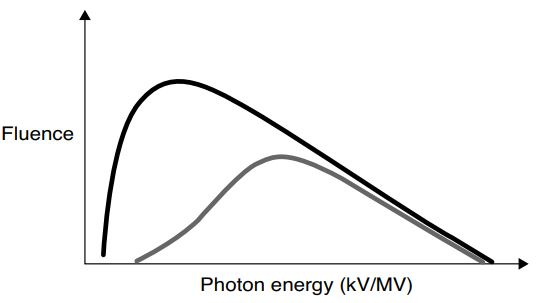
\includegraphics[width=0.5\textwidth]{Imagens/endurecimentoDoFeixe.JPG}
        \end{center}

        \item O output em um tubo de raios X kV é proporcional à corrente do tubo, porporcional ao quadrado da tensão do tubo e exponencialmente proporcional à corrente do filamento.
        
        \item O Cerrobend utilizado na confecção dos blocos em radioterapia é uma liga de bismuto, chumbo, estanho e cádmio. É útil como um material de alta densidade (\qty{9.4}{g/cm^3} ) e alto Z com um baixo ponto de fusão para criar rapidamente um bloco na forma desejada. O objetivo é atingir menos de 5\% de transmissão do feixe primário, o que significa 4.3 camadas semi-redutoras de cerrobend ou mais. 
        
        \item Um filtro físico também chamado de filtro em cunha, é formado por um material metálico com formatro triangular que gera um gradiente de intensidades do feixe na profundidade. Isso filtra diferencialmente os raios X de baixa energia, levando ao endurecimento do feixe. O grau de endurecimento do feixe é mais pronunciado perto do “calcanhar” mais grosso do filtro. Um filtro físico também é responsável pelo aumento do espalhamento da radiação.
        
        \item Um filtro virtual não produz endurecimento de feixe variável, pois o perfil de gradiente é criado pela abertura lenta de uma mandíbula do colimador do acelerador linear, em vez da transmissão através de Um filtro físico. Qualquer espalhamento pela mandíbula é reduzido pela blindagem no cabeçote da máquina e não contribui significativamente para a dose recebida pelo paciente.
        
        \item Quanto a distribuição espacial dos fótons produzidos por bremsstrahlung, para energias de elétrons incidentes na ordem de kV, os raios X são produzidos isotropicamente (em todas as direções). Com energias de elétrons incidentes da ordem de megavolt (MV), a distribuição de raios-X torna-se progressivamente mais alinhada com a direção dos elétrons incidentes. Portanto, um tubo de raios-X kV pode usar um alvo de reflexão onde os raios-X úteis estão a 90° do feixe de elétrons, enquanto um acelerador linear MV usa um alvo de transmissão onde os raios-x úteis serão emitidos aproximadamente na direção da velocidade dos elétros que incidem o alvo.

        \item Um filtro Thoraeus é comumente usado com tubos de raios-X de diagnóstico. O filtro consiste em camadas de estanho, cobre e alumínio para remover fótons de baixa energia e raios X característicos do feixe primário. Esses fótons de baixa energia não contribuem para a qualidade da imagem, mas aumentam a dose do paciente.
        
        \item A ordem das camadas do filtro Thoraeus é importante porque o estanho é o que mais contribui para a filtração dos raios X característicos do alvo de tungstênio, que ficam entre 58 keV e 69 keV. Os raios X característicos do estanho são de energia muito baixa e podem ser filtrados com cobre. Os raios X característicos do cobre são filtrados por uma fina película de alumínio, levando a um feixe endurecido capaz de produzir imagens nítidas.
        
        \item As interações de Bremsstrahlung ocorrem quando um elétron de alta energia passa perto do núcleo de um átomo. O elétron é desviado de sua trajetória original pelo núcleo devido à sua força coulombiana. O elétron sofre aceleração repentina em uma direção diferente (desacelerado), fazendo com que o elétron perca toda ou parte de sua energia nesse processo, que é convertida em um fóton. Um único elétron pode passar por múltiplas interações de bremsstrahlung antes de finalmente parar.
        
        \item Feixes de fótons de alta energia são criados por interações bremsstrahlung e, portanto, contêm um espectro de energia. A energia mais provável é aproximadamente um terço da energia máxima, que por convenção é usada para nomear o feixe (Energia nominal). Portanto, para um feixe de 10 MV a energia máxima é de 10 MeV e a energia mais provável é de aproximadamente 3,33 MeV. Isso não é o mesmo que a energia média, que é mais difícil de calcular.
        
        \item A filtração inerente em um acelerador linear é normalmente causada pelo próprio alvo de tungstênio (conforme os elétrons interagem com o alvo, um espectro de fótons é criado por meio de interações bremsstrahlung). Os fótons de baixa energia produzidos podem interagir e ser absorvidos pelo tungstênio remanescente antes de emergir para fora do alvo como parte do espectro. Este efeito aumenta à medida que a espessura do alvo aumenta. 
        
        \item A filtragem adicional é intencionalmente colocada no caminho de um feixe com o objetivo de aumentar a energia média do feixe (causando o endurecimento do feixe) ou diminuir a intensidade de um feixe.
        
        \item A penumbra do feixe (umbra é latim para “sombra”) é a redução gradual da intensidade do feixe na borda de um campo de fótons. É tipicamente medido como a largura entre as linhas de isodose de 80\% e 20\%, embora também sejam usadas linhas de isodose de 90\% a 10\%.
        
        \item Existem três fontes principais de penumbra do feixe que são a penumbra de transmissão, a penumbra geométrica e a penumbra interna. A penumbra de transmissão ocorre quando o feixe passa pela borda dos jaws, blocos ou colimadores multilâminas (MLC). A penumbra geométrica ocorre porque a fonte não é uma fonte pontual. A penumbra interna ocorre devido ao espalhamento dentro do paciente.
        
        \item O Cobalto-60 gera um feixe quase monoenergético (1,17 MeV, 1,32 MeV combinados para uma média de 1,25 MeV) e, portanto, o HVL1 = HVL2 = HVL3. No entanto, os tubos de diagnóstico usam a geração de raios-X bremsstrahlung para produzir um espectro de energias. Depois que o feixe passa pelo primeiro HVL, devido ao conceito de “endurecimento do feixe”, o segundo HVL agora é maior que o primeiro.
        
        \item A intensidade dos raios-X tem um pico direto (forward peaked) após o alvo e antes do filtro aplanador. O filtro aplanador é mais espesso no meio e afunila em direção às bordas, de modo que a região central seja atenue mais o feixe do que a periferia do filtro para tornar o feixe plano em uma profundidade específica. Como resultado, o feixe será mais endurecida no centro do que na periferia (menor energia média na periferia). Isso resulta em um feixe que atinge profundidades superiores a 10 cm. O filtro aplanador também reduz significativamente a taxa de dose.
        
        \item O feixe plano é especificado a 10 cm de profundidade e dentro da área delimitada por 80\% do tamanho do campo ou 1 cm dentro da borda do campo. A planicidade do feixe deve estar dentro de +–3\% da dose do eixo central a 10 cm de profundidade.
        
        \item Um filtro inclina as linhas de isodose em direção à sua borda fina. O ângulo entre o eixo central e as linhas de isodose a 10 cm de profundidade é o ângulo do filtro.
        
            \begin{center}
                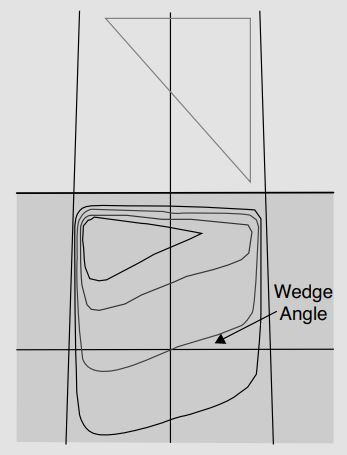
\includegraphics[width=0.5\textwidth]{Imagens/distruibuicaoDoseFiltro.JPG}
            \end{center}

        \item Feixes opostos paralelos são freqüentemente usados em radioterapia. Eles fornecem distribuição de dose uniforme para o alvo com uma configuração simples e reprodutível. Uma desvantagem dessa técnica é chamada de “efeito lateral do tecido”. O ponto médio entre os feixes opostos é o ponto de prescrição. A relação entre a dose máxima e a dose do ponto médio (ponto de prescrição) aumenta com a espessura do paciente e diminui com a energia. Como resultado, é melhor usar feixes de raios X de maior energia (>10 MV) para pacientes grandes (>20 cm) para melhorar a homogeneidade da distribuição da dose e preservar o tecido subcutâneo.
        
        \item A dose integral é simplesmente massa x dose se a dose for uniforme em toda a região, ou a soma da energia depositada. Se for calculado o histograma de volume de dose, a dose integral é a área sob o contorno externo, que inclui todo o tecido do paciente. A unidade de “dose integral” é kg/Gy ou joule. É usado para determinar a qualidade do plano de tratamento em relação à quantidade de dose administrada fora do alvo. A dose integral diminui com a energia.
        
        \item Novos aceleradores lineares (linacs) estão disponíveis com feixes FFF. Os Linacs requerem um filtro aplanador para produzir feixes planos em grandes campos abertos. No entanto, o filtro aplanador reduz a taxa de dose da máquina e produz o endurecimento do feixe. Com tratamentos de radioterapia com intensidade modulada (IMRT) para campos pequenos , os colimadores multilâminas (MLCs) são usados para modular deliberadamente a intensidade do feixe. Para esses tratamentos, o filtro não é mais necessário. As vantagens dessa abordagem incluem uma taxa de dose significativamente aumentada (>1.000 MU/min versus 300 a 600 MU/min) e e diminuição da variação no espectro de energia produzido(que é maior para feixes plano devido ao endurecimento do feixe). As desvantagens dessa abordagem incluem um possível aumento na dose da pele (menor endurecimento do feixe aumentando a quantidade de fótons de baixa energia) e a incapacidade de tratar campos grandes, planos e abertos sem o uso de MLCs. Alguns fabricantes adicionam um filtro fino para remover fótons de energia muito baixa para feixes não planos.
        
        \item A “energia efetiva” é definida como a energia de um feixe de raios X monoenergético que tem a mesma camada semi-redutora que o feixe heterogêneo de raios X.
        
        \item O valor da Porcentagem de dose na profundidade (PDP) a 10 cm de profundidade para um tamanho de campo de 10 cm x 10 cm com distância da fonte à pele de 100 cm é usado para definir a qualidade do feixe.
        
        \item Diferentemente dos fótons, as energias dos elétrons são escritas como megaelétrons volts (MeVs) porque as energias de elétrons são monoenergéticas quando deixam o guia de ondas acelerado, mas os fótons apresentam um feixe polienergético. A energia do fóton MV representa o raio-X de maior energia (em MeVs) no espectro.

    \end{itemize}

    \textcolor{CarnationPink}{Fatores que Afetam a deposição de dose pelos fótons}
    \begin{itemize}
        \item Para um determinado tamanho de campo, a PDP (expressa em porcentagem) é medida ao longo do eixo central e é definida como a razão de uma dose em uma determinada profundidade d para a dose em uma profundidade de referência (geralmente d\textsubscript{max}) no eixo central.
        
            $$PDP = \frac{Dose\;na\;profundidade\;d}{Dose\;na\;profundidade\;de\;referencia\;d_{max}} \times 100\%$$

            $$PDP(d) = \frac{D(d)}{D(d_{max})} \times 100\%$$

        \item A PDP em uma produndidade d pode ser afetada por variaçoes no tamanho de campo, energia, SSD e pela utilização de filtros da seguinte maneira:
        
            \begin{enumerate}[label=\roman*)]
                \item Com o aumento do tamanho de campo, a PDP(d) irá aumentar devido ao aumento do espalhamento no meio.
                \item Cpm Aumento da energia do feixe, a PDP(d) irá aumentar devido ao aumento da penetração;
                \item Com o Aumento da SSD a PDP(d) irá aumentar devido à lei do inverso quadrado, pois a dose em $d_{max}$ irá diminuir.
                \item Com a inserção de um filtro físico ocorrer o endurecimento do feixe e portanto ocorrerá um aumento na PDP. 
            \end{enumerate}

        \item A curva de PDP relata a deposição de dose em função da profundidade de um feixe de radiação. O PDP na superfície para energias de megavoltagem está abaixo de 100\%, pois os fótons incidentes produzem elétrons de alta energia que percorrem uma distância antes de parar e depositar energia. Este efeito explica as propriedades de “skin sparing” da terapia de megavoltagem. O pico na curva conhecida como D\textsubscript{max}, ocorre em uma maior profundidade. A curva então declina, ou atenua, devido a uma combinação da lei do inverso do quadrado, absorção e espalhamento.
        
        \begin{center}
            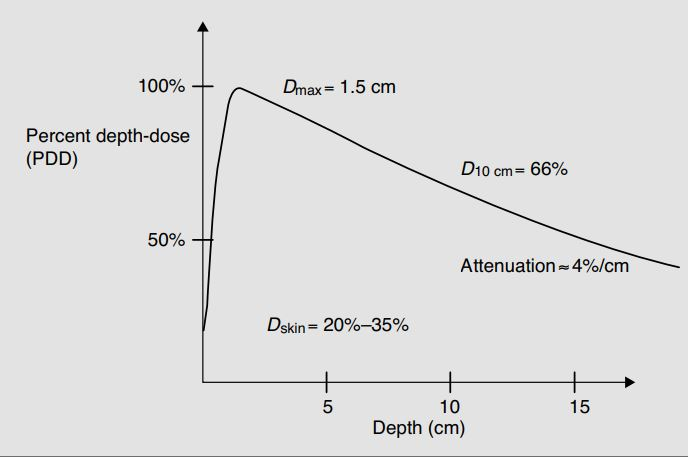
\includegraphics[width=0.5\textwidth]{Imagens/pdp.JPG}
        \end{center}

        \item Os valores de d\textsubscript{max} são sutilmente diferentes para cada máquina e feixe, porém os valores tipicos para cada energia nominal são:
        
            \begin{enumerate}[label=\alph*)]
                \item \ce{^{60}Co}: 0.5 cm;
                \item 6 MV: 1.5 cm;
                \item 10 MV: 2.5 cm;
                \item 15 MV: 3.0 cm;
                \item 18 MV: 3.2 cm até 3.5 cm
            \end{enumerate}

        \item Sob as condições de referência, um feixe de \ce{^{60}Co} atenua aproximadamente 4\% por cm.  Feixes de Fótons de 6 MV atenuam aproximadamente 3.5\% por centímetro. E Feixes de 10 MV atenuam aproximadamente 3.3\% por centímetro. Esses valores são uma aproximação, pois os valores de atenuação mudam com a produndidade.
        
        \item Normalmente, os valores de PDP ou TMR são tabelados apenas para campos quadrados. Um campo retangular terá aproximadamente a mesma PDP ou TMR que seu campo quadrado equivalente. Existem também outros métodos mais complexos para aproximar a PDD ou a TMR para formas de campo irregulares, como o método de Clarkson.
        
        \item A PDP é normalmente determinada para valores de SSD de 100 cm. Para estimar a PDP para diferentes valores de SSD é utilizado o Fator de Mayneord (F). o Fator F é uma estimativa das mudanças na PDP causadas apenas pela lei do inverso quadrado. Este fator assume que a quantidade de espalhamento é constante a medida que a SSD muda, o que não é correto e portanto limita a precisão deste método. Para baixas energias, a correção da razão tecido-ar (TAR) para o método do fator Mayneord F pode ser usada se as tabelas TAR estiverem disponíveis.
        
        \item O tamanho do campo é normalmente definido no isocentro da máquina, a 100 cm da fonte. Isso seria, então, na superfície do paciente para a configuração da distância da fonte à pele (SSD) ou no isocentro para a configuração da distância da fonte ao eixo (SAD).
        
        \item Fotons com energias superiores a 10 MV não são recomendados para o tratamento de câncer de pulmão. A diferença na densidade eletrônica entre o pulmão e o tecido mole ou osso da parede torácica apresenta problemas especiais no manejo do câncer de pulmão. Fótons de alta energia podem contribuir para aumentar a dose espalhada no pulmão. Além disso, a maior região de build-up para fótons de alta energia pode comprometer a cobertura do tumor em sua periferia.
        
        \item A região de buildup é a região inicial na curva de PDP, entre a superfície do paciente e d\textsubscript{max}. A deposição de dose pelos fótons depende de elétrons secundários. Enquanto os fótons são constantemente atenuados exponencialmente em função da lei do quadrado inverso, os fótons de alta energia requerem alguma profundidade no tecido para gerar elétrons secundários, explicando assim porque a dose depositada é baixa na superfície do tecido irradiado.
        
        \item A profundidade de d\textsubscript{max} diminui ligeiramente em função do tamanho do campo. Por exemplo, um d\textsubscript{max} de 1,5 cm é estimado para um fóton de 6 MV e um campo de 10 cm x 10 cm, enquanto para um campo de 20 cm x 20 cm esperasse uma  d\textsubscript{max} de 1,4 cm. Isso se deve ao aumento do espalhamento que contribui para a deposição superficial da dose, aproximando d\textsubscript{max} da superfície.
        
        \item A PDP aumenta à medida que o tamanho do campo aumenta devido ao espalhamento no tecido fora do eixo central (off-axis). Tanto a dose primária (fótons emitidos diretamente do cabeçote do linac) quanto a dose secundária (espalhamento no tecido) contribuem para a PDP. Embora tanto a dose na profundidade d (D\textsubscript{d}) quanto a dose em d\textsubscript{max} aumentam, o D\textsubscript{d} aumenta mais que a dose em d\textsubscript{max}(D\textsubscript{max}), portanto a PDP aumenta.
        
        \item O aumento da PDP com o tamanho de campo é maior para feixes de baixa energia. Com altas energias, a maior parte do espalhamento ocorre na mesma direção do fóton incidentee portanto o espalhamento lateral é menor.
        
        \item As maiores vantagens em se utilizar a técnica SAD (que utiliza o fator TMR) quando comparado a técnica de SSD (que utiliza o fator PDP) é que os cálculos utilizando a PDP são convenientes quando não há mudanças na SSD e a SSD é mantida na distância padrão de calibração igual a 100 cm. No entando, um tratamento com diversos campos, a SSD irá mudar devido a variações na superfície do paciente, ou então o paciente deverá ser movido em todo campo de tratamento para igualar a SSD à SSD de calibração. Ao utilizar o método de SAD, utiliza-se a TMR ao invés da PDP, e como a TMR é independente da SSD, torna-se uma vantagem nessas situações de SSD variáveis. 
        
        \item A Razão Tecido-AR (TAR - tissue-to-air ratio) é definida como a dose em um ponto no tecido dividida pela dose no ar no ponto com a mesma distancia à fonte. Devido a distância até a fonte para ambas componentes da razão serem as mesmas, a TAR não varia com a SSD, fornecendo uma vantagem para cálculos com a SSD variável (vários campos com setup SAD). Se o campo aumenta, mantendo a profundidade constante, haverá mais espalhamento no tecido, e portando o termo do numerador irá aumentar. No entanto, não há espalhamento no ar e o denominador se mantém constante, levando a um aumento na TAR. Uma vez que altas energias são mais penetrantes no tecido, a TAR aumenta com o aumento na energia.

            \begin{center}
                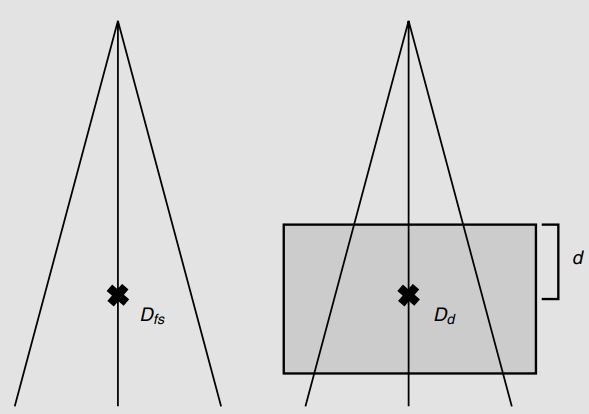
\includegraphics[width=0.5\textwidth]{Imagens/tar.JPG}
            \end{center}
        
        \item O diagrama abaixo mostra a relação entre a Porcentagem de Dose na profundidade (PDP) a  Razão Tecido-Ar (TAR) a Lei do Inverso Quadrado (ISL) e o fator de espalhamento de pico (PSF) que é definido como a TAR na produndidade de dose máxima d\textsubscript{max}:
        
            \begin{center}
                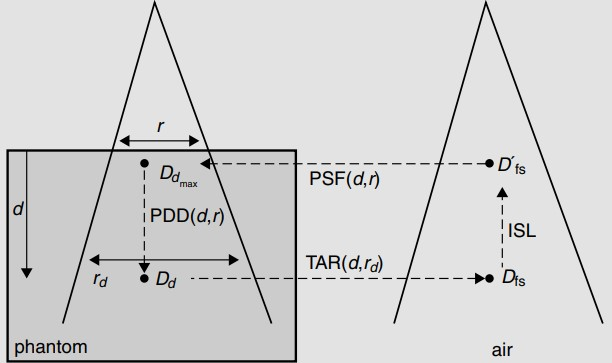
\includegraphics[width=0.5\textwidth]{Imagens/relacoes.jpg}
            \end{center}        
            
            $$D_d = \frac{PDP(SSD, D, r) \times D_{max}}{100}$$

            $$D_{fs} = \frac{D_d}{TAR(d, r_d)}$$

            $$D_{fs}' = \sqrt{D_{fs}^2\left(\frac{SSD}{SSD + d}\right)^2}$$

            
            $$D_{d_{max}} = PSF(r) \times D_{fs}'$$
        
        \item O fator BSF (backscatter factor) é um caso especial da PSF (peak scatter factor) quando fótons de baixa energia com um d\textsubscript{max} igual a zero são considerados. Se d\textsubscript{max} é perto de zero, o único espalhamento que contribui para dose em d\textsubscript{max} é devido ao retroespalhamento, e por isso o nome ``backscatter''. 


        \item Uma vez que os fótons de alta energia tendem a espalhar ``para frente'' o PSF diminui em apenas poucos por cento para feixes de alta energia (PSF varia de 1.05 até 1.1). O PSF, ou mais precisamente, o fator de retroespalhamento é maior para fótons de baixa energia devido ao aumento do espalhamento lateral no tecido (pode ser mais alto em aproximadamente  40\% a 50\% para feixes de diagnóstico).
        
        \item A TMR é dada pela equação:
        
            $$TMR(d) = \frac{D(d, SAD)}{D(d_{max}, SAD)}$$

            Neste caso as doses são calculadas nas profundidades d e $d_{max}$ e ambas possuem a mesma distância até a fonte (portando o ponto deve ser posicionado na distância de referencia)
        
            \begin{center}
                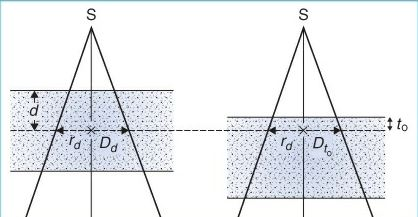
\includegraphics[width=0.5\textwidth]{Imagens/tmr}
            \end{center}

        \item A TMR está relacionada com a TAR a partir do PSF:
        
            $$TMR = \frac{TAR}{PSF}$$

        \item A diferença entre a PDP e a TMR é que, embora ambas sejam dadas pela razão entre a dose no ponto e a dose na profundidade máxima, A PDP é calculada utilizando a mesma Distância da Fonte até a Superfície (SSD) em profundidades diferentes enquanto que o TMR é calculado utilizando a mesma distância da fonte ao eixo (SAD) e portanto é independente da SSD. 
        
        \item Em pacientes que irão tratar regiões onde á irregularidades na superfície da pele,; uim bolus pode ser colocado na superfície da pele para uniformizar a irregularidade da superfície do paciente. A adição de um bolus removerá, no entanto, o efeito poupador da pele da radiação de megavoltagem. Alternativamente, filtros compensadores podem ser usados. Um filtro compensador atenua o feixe na região do “tecido ausente”. Outras técnicas para controlar as irregularidades da superfície incluem o uso de filtros em cunha ou o blindagem de partes do tecido em algumas das frações do tratamento.
        
        \item O tamanho de campo é definido pela linha de isodose de 50\%. O tamanho de campo muda com a distância devido a divergencia do feixe e então é definido no isocenteo da máquina.
        
        \item O método de Clarkson é utilizado para calcular a dose para campos irregulares. Esta técnica envolve dividir um campo irregular em diversas regiões para aproximar o espalhamento para cada região. 
    \end{itemize}

    \textcolor{CarnationPink}{Cálculo de Unidades Monitoras}
    \begin{itemize}
        \item As condições de referência são as condições nas quais o feixe é calibrado. É extremamente importante especificar essas condições, caso contrário, podem ocorrer erros sistemáticos nos cálculos de dose. Um exemplo de condições de referência comuns é que o feixe pode ser calibrado (de acordo com AAPM TG-51) de modo que 1 unidade monitora (1 MU) seja igual a dose de 1 cGy depositada por um fóton de 6 MV na profundidade d\textsubscript{max} usando um tamanho de campo de 10 cm x 10 cm em água com uma distância da fonte à superficie (SSD) de 100 cm. Observe que o tamanho do campo é determinado a 100 cm da fonte.
        
        \item A dose em um ponto na profundidade é dada pela soma da dose devido à radiação primária (proveniente do feixe primário emitido pelo acelerador) e a dose espalhada proveniente do espalhamento dentro da máquina ou dentro do paciente.
        
        \item $S_c$ é o fator de espalhamento do colimador e $S_p$ o fator de espalhamento do phantom (tecido). Os fótons que interagem com objetos presentes no cabeçote do acelerador, como o alvo, o filtro aplanador, os jaws colimadores, tendem a se espalhar e entrar no paciente em vários ângulos (Sc). Uma vez que os fótons entram no paciente, eles são espalhados novamente (Sp). Sc e Sp são principalmente uma função do tamanho de campo, uma vez que mais espalhamento ocorre em aberturas de campo maiores. Como são fatores de correção, eles são tipicamente próximos de 1, mas podem variar de 0,9 para campos pequenos a 1,1 para campos grandes. Às vezes, para simplificar, eles são combinados em um único termo, $S_{c,p}$, que é simplesmente Sc x Sp. Observe que o tamanho do campo para $S_c$ é definido no isocentro. No entanto, o tamanho do campo para $S_{p}$ é definido na profundidade, uma vez que o espalhamento interno pode mudar à medida que o feixe diverge com a profundidade.
        
        \item O fator $S_c$ é definido como a razão entre o output para um dado tamanho de campo e o output para o campo de referência (10 cm x 10 cm) ambos medidos no ar no isocentro (100 cm). Esta medida é feita com uma câmara de ionização com uma capa de build-up.
        
        \item o fator $S_p$ é a razão entre a taxa de dose para um determinado tamanho de campo e a taxa de dose  para o tamanho de campo de referência (10 cm x 10 cm) medida em um phantom na profundidade $d_{max}$ ou profundidade de referência com abertura de colimador idêntica. Teoricamente, poderia ser medido usando fantomas de vários tamanhos com uma abertura de colimador maior. Mas, na prática, é medido indiretamente usando a seguinte equação:
        
            $$S_p(r) = \frac{S_{c,p}(r)}{S_c(r)}$$

        onde $S_{c,p}(r)$ é o fator de espalhamento total definido como a taxa de dose na profundidade de referência para um dado tamanho de campo r dividido pela taxa de dose no mesmo ponto e profundidade para o campo de referência. o $S_{c,p}(r)$ normalmente é medido em profundidades de referência maior que $d_{max}$ para evitar a contaminação com eletrons e então é convertido para $d_{max}$ através da PDP.

        \item De acordo com o TG-71, o cálculo de MU para o setup SSD simplificado (sem considerar Fator Off-axis, fator filtro e demais modificadores de feixe) é dado através da seguinte equação:
        
            $$MU = \frac{D}{D_0' \cdot S_c(r_c) \cdot S_p(r_{d}) \cdot PDP_N(d, r, SSD) \cdot \left(\frac{SSD_0 + d_0}{SSD + d_0}\right)^2}$$

            \begin{itemize}[label=\textopenbullet]
                \item $D$: A dose no ponto de interesse.
                \item $D_0'$: Dose por UM em condições de calibração.
                \item $d$: Profundidade do ponto de cálculo.
                \item $d_0$: A profundidade de normalização para dosimetria de fótons e elétrons, normalmente $d_{max}$.
                \item $r_c$: O lado do quadrado equivalente para o tamanho do campo do colimador definido no isocentro.
                \item $r_d$: O lado do quadrado equivalente para o tamanho do campo incidente no paciente, definido na superfície e na profundidade d, respectivamente.
                \item $S_c$: Fator de dispersão do colimador.
                \item $S_p$: fator de dispersão do phantom 
                \item $PDP_N$: é a PDP / 100.
            \end{itemize}

        \item De Acordo com o TG-71, o cálculo de MU para o setup SAD é dado por:
        
            $$MU = \frac{D}{D_0' \cdot S_c(r_c) \cdot S_p(r_{d}) \cdot TPR(d, r_d) \cdot WF(d, r_d, x) \cdot TF \cdot OAR(d, x) \cdot \left(\frac{SSD_0 + d_0}{SPD}\right)^2}$$

            \begin{itemize}[label=\textopenbullet]
                \item $SPD$: é a distancia do ponto até a fonte;
                \item $TPR$: é a razão tecido máximo;
                \item $TF$: é o fator de transmissão;
                \item $WF(d, r_d, x)$: é o fator filtro na produndidade d a uma distância x do eixo central;
                \item $OAR(d, x)$: é o fator off-axis para uma distância x do eixo central.
            \end{itemize}

        \item Uma “regra de ouro” é que o cobalto-60 decai aproximadamente 1\% ao mês. Embora esta seja uma boa resposta a ser lembrada para estimativa, ela não funcionará por um longo período de tempo. A resposta precisa, é utilizando a lei de decaimento exponencial com o tempo de meia vida de 5.26 anos e o tempo de análise igual a 1 mês. 
        
        \item As máquinas de Cobalto-60 apresentam maior penumbra geométrica devido a fonte de cobalto ser normalmente um cilindro com diâmetro variando entre 1cm a 2cm, diferentemente do diâmetro do feixe estreito de elétrons utilizado nos aceleradores lineares que possui diâmetro de aproximadamente 3 mm ao interagir com o alvo de tungstênio.
        
        \item Os equipamentos de Cobalto-60 são controlados através de um timer. Devido a fonte estar sempre ``ligada'', pois se trata de um material radioativo, a fonte é sempre mantida dentro de uma blindagem no cabeçote da máquina e a blindagem só é removida no momento em que o paciente está sendo tratado. A calibração de uma bomba de cobalto é ralizada então atraves da medida do tempo que leva para uma fonte depositar sua dose, no qual é uma função da atividade da fonte. Uma fonte mais nova tem tipicamente uma taxa de dose de 240cGy/min na SAD de 80 cm.

        \item A correção de tempo em tratamentos com cobalto-60 leva em conta o tempo que leva para afastar a blindagem da fonte de cobalto. Por uma fração desse tempo, a fonte não está totalmente exposta e não está fornecendo a taxa de dose total. Portanto, o erro de tempo é adicionado ao tempo que leva para entregar a fonte.

    \end{itemize}
\end{exemplo}

\begin{exemplo}[6. Básico de Planejamento de Tratamento]
    \begin{itemize}
        \item Em um tratamento de crânio total (WB) normalmente são utilizados dois campos laterais deslocados \ang{5} para a direção anterior do paciente, resultando em um campo com angulação de \ang{275} e um campo com angulação de \ang{85}. Este deslocamento no ângulo do gantry é feito para evitar a divergência do feixe nos cristalinos, minimizando a dose depositada nessas estruturas. 
        
        \item O belly board é um acessório de imobilização comumente utilizado em tratamentos de cancer retal. O belly board consiste em um ``colchão'' com uma cavidade em seu centro que permite que o paciente deite em uma posição pronada e toda a cavidade abdominal fique dentro da cavidade do acessório. Isto faz com que o intestino de desloque para uma posição mais anterior do paciente e então distancia o intestino do volume alvo, reduzindo a dose de radiação no intestino; 
        
        \item Outra técnica frequentemente utilizada para diminuir a dose no intestino delgado é diminuindo a proporção de intestino dentro do campo é tratar o paciente com a bexiga cheia. Nestes casos, a bexiga irá empurrar o tumor inferiormente e semparar o intestino do volume de tratamento.
        
        \item Um bolus é qualquer material adicionado sobre a superfície do paciente ou próximo a superficie e normalmente é feito de um material agua-equivalente. O bolus pode ser utilizado para aumentar a dose na superfície em tratamentos de lesões mais superficiais ou também pode ser uitilizado para compensar a falta de tecido em tratamentos como o de uma órbita ocular quando o globo ocular foi removido.
        
        \item Em planos de tratamento de Radioterapia, um ponto quente é definido como um pequeno volume que recebe a maior dose de radiação, sendo essa dose maior que a dose de prescrição para o alvo. Na Radioterapia Convencional, antes de serem utilizados cálculos 3D e imagens 3D, ou seja, nas técnicas 2D, um ponto quente era definido para uma area que engloba \qty{2}{cm^2} de área contígua que recebe a maior dose de radiação. Na Radioterapia conformacional 3D, o ponto quente é definido como o volume (0.03mL) recebendo a maior dose de radiação.
        
        \item Em um campo AP/PA utilizado para um tratamento na região do tórax prescrito no meio do DAP (Distância Ântero-Posterior), como a medula está localizada posteriormente, o maior tamanho de medula recebendo dose de radiação será devido ao campo anterior. Como o campo anterior está mais distânte da medula, devido à divergência do feixe, o tamanho de campo na medula será maior para o campo anterior do que para o campo posterior, que está mais próximo a medula. O tamanho de campo só será o mesmo para o Anterior e para o posterior no isocentro definido no meio do DAP. 
        
        \item A principal vantagem em utilizar a técnica isocêntrica em tratamentos com multiplos campos ao invés da técnica da SSD é que a técnica isocentrica elimina a necessidade de movimentação do paciente para cada campo de tratamento. Na técnica SAD, O isocentro é colocado dentro do paciente na profundidade planejada e os feixes incidem a partir de diferentes ângulações direcionadas para o mesmo ponto. Esta técnica depende principalmente da precisão da isocentricidade da máquina e não das marcas na pele no paciente, como é o caso dos tratamentos via SSD, que podem ser pontos de referência não confiáveis.

        \item Em pacientes de mama, pode-se optar pelo posicionamento do paciente em decúbito ventral. Este tratamento apresenta vantagens nos casos em que a cavidade tumoral está afastada da parede torácica ou quando a paciente possui mama pendular. Nestas situações o posicionamento em decúbito ventral ajudará a diminuir a dose nos pulmões e no coração. Outra técnica utilizada para reduzir a dose no coração em tratamentos de mama esquerda é a técnica de inspiração profunda (breath-hold), que faz com que a região cardíaca seja afastada da parede toráxica reduzindo significativamente a dose recebida no coração comparado à inspiração livre. 
        
        \item Em um planejamento de mama total utilizando campos tangentes, a separação é um parâmetro que auxilia na escolha da energia do feixe de tratamento. A separação é definida como a distância entre as entradas dos dois campos tangentes. Se a separação exceder 23 cm, o aumento da energia do feixe de 6 MV para 10 MV poderá melhorar a uniformidade da distribuição de dose dentro da mama, podendo ficar $>$ que 110\% da dose prescrita. 

        \item Ao criar gaps em tratamentos de neuroeixo, onde s campos se interceptam na ponfudidade, o ponto quente irá ocorrer na região abaixo do gap, abaixo da profundidade de interseção dos campos enquanto os pontos frios ocoorem na região abaixo do gap, acima da profundidade de interseção dos campos. Para minimizar os efeitos dos pontos quentes e frios que ocorrem no neuroeixo, realiza-se o deslocamento do gap, alterando a posição das bordas do campo entre as frações durante o curso de tratamento. Desta forma os pontos quentes e frios são movidos para regiões diferentes, diluindo o efeito desses pontos. 

        \item No ponto de junção, a dose para cada campo é igual a 50\% da dose de prescrição na mesma profundidade de cada campo. Desta forma é alcançada uma uniformidade da dose em toda area de tratamento na mesma profundidade. 
        
        \item Um diagrama para determinar o tamanho do gap na superficie da pele para um tratamento de neuroeixo é apresentado da figura abaixo:
            \begin{center}
                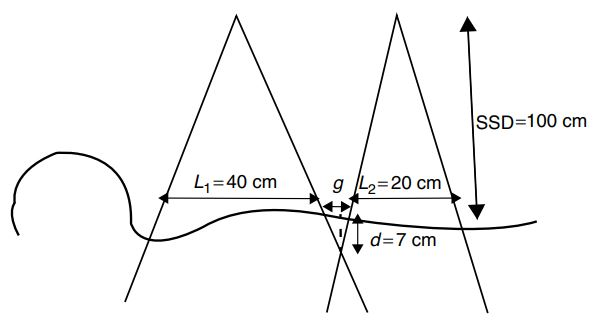
\includegraphics[width=0.5\textwidth]{Imagens/gapNeuroEixo.JPG}
            \end{center}
        
        \item No neuroeixo, são utilizados campos para tratar o crânio e campos para tratar a coluna. Caso os campos do crânio sejam não divergentes (utilizando a técnica de tenham meio campo bloqueado), então o colimador deverá girar em uma angulação que seja suficiente para ocorrer uma coincidencia geométrica entre o campo do crânio e o campo da coluna. Caso o feixe do crânio seja divergente, então além da angulação do colimador, também será necessário uma angulação da mesa em direção ao gantry para coincidir as divergências do feixe. 
        
        \item A figura abaixo representa o esquema para definição do ângulo de rotação do colimanor necessário para coincidir as divergências dos feixes:
        
            \begin{center}
                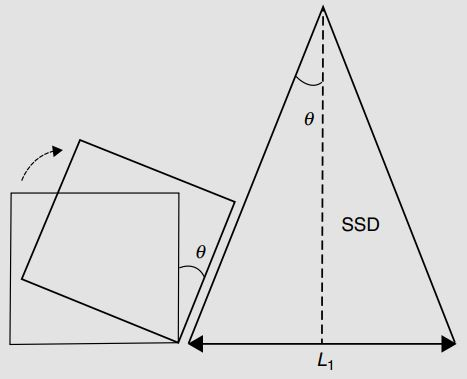
\includegraphics[width=0.5\textwidth]{Imagens/divergenciaColimador.JPG}
            \end{center}
        
        \item A figura abaixo representa o esquema para definição do ângulo de rotação da mesa  necessário para coincidir as divergências dos feixes do crânio com a coluna:
        
            \begin{center}
                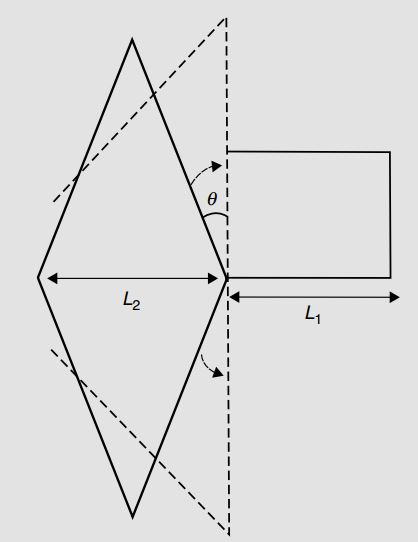
\includegraphics[width=0.5\textwidth]{Imagens/divergenciaMesa.JPG}
            \end{center}

        \item Um feixe de fótons de 10 MV, ao atravessar uma distância no pulmão, há um aumento na dose além do decido pulmonar de aproximadamente 2\% por cm de pulmão atravessado.
        
        \item Em um tratamento de mama com tangentes, não é recomendado utilizar filtros físicos na tangente interna caso seja desejável diminuir a dose espalhada na mama contralateral. 
        
        \item A técnica de tangente ampla é utilizada em tratamentos de mama que incluem a mamária interna, onde a tangente interna é definida de modo que a borda do campo é aberta no sentido da mama contralateral para englobar a mamária interna, enquanto a tangente externa abrange todo o tecido mamario. Porém, caso a configuração dos campos englobe muito tecido pulmonar, o recomendado é utilizar um campo separado de elétrons que case com as tangentes para reduzir a dose no pulmão. 
        
        \item Segundo o ICRU O GTV (Gross tumor volume) é o tumor visível em uma imagem e examinação física; O CTV (clinical target volume) é a região com risco de disseminação subclínica (microscópica); O ITV (integrated target volume) adiciona margens para considerar movimentaçõos conhecidas do tumor, devido à respiração por exemplo; O PTV (planning target volume) adiciona margens para considerar os erros aleatórios no setup do paciente. Portanto em ordem de tamanho do menor volume para o maior temos: $GTV < CTV < ITV < PTV$.
        
        \item O Volume tratado (Treated Volume - TV) é o volume coberto com a isodose de prescrição. O volume irradiado (Irradiated Volume - IV) é o volume coberto por 50\% da  isodose de prescrição

        \item De acordo com o ICRU a precisão da entrega da dose deve estar dentre $\pm 5\%$ do esperado. 

        \item A técnica do Four-Field Box (4 campos) é uma técnica de planejamento de tratamento onde quatro campo espaçados por uma angulação de \ang{90} entre si, contendo um campo anterior, um campo posterior, um campo lateral direito e um campo lateral esquedo que formam uyma distribuição de dose com formato quadrado ou retangular semelhante a uma caixa; Estes camos eram tipicamente utilizados para tratamentos de próstata antes da vinda do IMRT. 
        
        \item Para ocorrer um match entre campos adjacentes de fótons, o método mais típico é utilizando campos meio-bloqueados e realizar o match no isocentro onde não haverá divergência do feixe. Outra forma é combinando as divergências dos campos adjascentes angulando os campos um em relação ao outro, podendo utilizar angulações de mesa, colimador e gantry. 
            
        \item Os principais algoritmos de cálculo de dose utilizados em sistemas de planejamento são o pencil beam, superposition convolution e Monte Carlo. O algoritmo pencil beam tem sido largamente eliminado devido a incapacidade de considerar com precisão as heterogeneidades do meio como o pulmão e outros tecidos moles.
        
        \item Em planejamentos 3D, ao tratar um alvo central, pode ser uma maneira mais simplista utilizar campos AP/PA, porém esta geometria irá irradiar a medula tanto quanto o alvo. Para reduzir a dose na medula, normalmente é adicionado um campo obliquo evitando a medula ``off cord''; O campo AP/PA é utilizado para tratar em torno de 40 Gy (até um pouco abaixo da tolerância da medula) e então o campo obliquo evitando a medula é utilizado para complementar a dose. 
        
        \item Em um tratamento com geometria AP/PA para tratar a medula, como a medula fica mais posterior, o peso do campo posterior que está mais próximo a medula é definido entre 60\% a 70\%.
        
        \item Em um tratamento com par de filtros, os filtros são planejados para que eles fiquem com sua parte mais grossa juntas. O par de filtros é utilizado para reduzir a dose onde há o maior overlap entre os dois campos na menor profundidade.
        
        \item Em um tratamento de mama, as posições típicas para as bordas do campo são:
        
            \begin{itemize}[label=\textopenbullet]
                \item Borda Superior - Definida 1 cm acima do tecido mamário no qual é normalmente logo abaixo da cabeça clavicular;
                \item  Borda Inferior - É definida a 2 cm abaixo da linha inframamária;
                \item  Borda Medial - É definida na linha média do tórax ou no meio do esterno;
                \item Borda Lateral - É definida na linha axilar média. 
            \end{itemize}
        
        \item A densidade do Cerrobend é cerca de 83\% da densidade do chumbo; O Cerrobend é composto de 50\% de bismuto, 26.7\% de chumbo 13.3\% de estanho e 10\% de cádmio. 
        
        \item Cerrobend pode ser dimensionado para atenuar qualquer quantidade de um feixe, dependendo de sua espessura. Tipicamente, o bloco de Cerrobend é feito de modo que permita a transmissão de 5\% ou menos. Para isto é necessário aproximadamente 4.3 HVL's.
        
        \item Os blocos de cerrobend são focados na direção da fonte de raios-x cortando-os de modo que correspondam à divergência do feixe. Quando os blocos são cortados, um molde de isopor é colocado em uma bandeja acima de um filme radiográfico ou uma DRR. Uma caneta presa a um fio aquecido fixado em um ponto distante do isopor igual à distancia da fonte ao bloco, é utilizada para traçar o contorno da forma planejada para o bloco de acordo com o filme abaixo. O fio aquecido é inclinado para coincidir com a divergência do feixe originário de uma fonte a essa distância enquanto corta o isobor. O isopor cortado é então utilizado como molde para despejar o cerrobend. 

        \item Os MLC são feitos de tungstênio e diferentemente dos blocos de cerrobend, os MLC's são focados apenas na direção perpendicular à direção de movimentação do MLC, e não são focados na direção paralela ao movimento do MLC. A penumbra na direção paralela ao movimento do MLC é maior quando comparada aos blocos moldados de cerrobend. Os MLC' possuem lâminas de bordas arredondadas para minimizar a transmissão parcial na borda da lâmina. Os blocos de Cerrobend também ficam mais perto do paciente que o MLC, reduzindo ainda mais a penumbra. 
        
        \item A transmissão do MLC pode variar dependendo do fabricante. Os valores tipos para a transmissão atraves do MLC é de aproximadamente 2\% a 4\% para a transmissão interlâmina (entre as lâminas); 1\% a 2\% para a transmissão intra-lâmina (através da lâmina) e de 15\% a 24\% para a transmissão nas bordas das lâminas. A transmissão interlâminas incluem o uso de arranjos steps in groove entre as lâminas (``degrau e ranhura''). A figura abaixo mostra exemplos de MLC com esse arranjo para diferentes fabricantes. 
        
            \begin{center}
                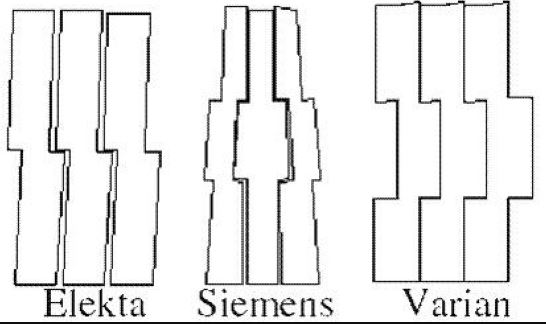
\includegraphics[width=0.5\textwidth]{Imagens/tongueInGroove.JPG}
            \end{center}
        
        \item Embora o feixe possa ser blindado com um bloco, ainda existirá dose na região abaixo ao bloco. Essa dose se deve a duas contribuições: A dose transmitida através do bloco e a dose espalhada pela região fora da região bloqueada. A dose embaixo do bloco é da ordem de 10\% da dose na região não bloqueada, dependendo da largura do bloco, pois um bloco mais estreito iria permitir mais espalhamento embaixo dele.


        \item Em tratamentos usando campos paralelos opostos com a dose prescrita no plano médio, a profundidade contendo a maior dose será na profundidade de dose máxima para essa geometria de campos. Para melhorar a uniformidade do plano, é ideal utilizar a maior energia de fótons disponível, pois quanto maior a energia, mais profunda é a penetração do feixe resultando em uma distribuição de dose mais uniforme. 
        
        \item Em campos filtrados, o ``hingle angle'' (ângulo da dobradiça) é a angulação entre os eixos centrais de dois campos filtrados. A figura abaixo mostra a definição do angulo hinge. 
        
            \begin{center}
                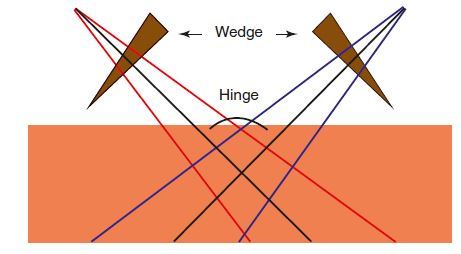
\includegraphics[width=0.5\textwidth]{Imagens/hinge.JPG}
            \end{center}
        
        \item Uma possibilidade de tratamento na pelve para tratamento de cancer retal é utilizadno a geometria de três campos compostos por dois campos laterais e um campo posterior, onde filtros podem ser utilizados para compensar a espessura diferencial do paciente a partir da região anterior para a posterior. Neste caso são utilizados filtros nos campos laterais, com a maior espessura do filtro no sentido posterior do paciente, apontando para a região do sacro pois esta região costuma ser mais fina que a região anterior. Outra vantagem de utilizar os filtros nessa posição é que permite reduzir os pontos quentes causados pela combinação dos campos laterais com o campo posterior.
        
        \item Em tratamentos de esôfago, normalmente é prescrita uma dose de 50,4 Gy. As possibilidades simples de tratamento são utilizando campos paralelos opostos AP/PA ou a técnica de 4 campos. A maior desvantagem em utilizar os campos paralelos opostos, é que a medula irá receber aproximadamente a dose prescrita ou até mesmo doses superiores pois os pontos quentes utilizando essa geometria estão mais perto da superficie do paciente. Este problema pode ser minimizado utilizando a geometria de 4 campos, porém sua maior desvantagem é que esta técnica resultará em uma maior dose nos pulmões. 
        
        \item A medida que o tamanho de campo aumenta, haverá uma maior contaminação de elétrons no feixe devido às interações de espalhamento com o colimador e com o ar, portanto haverá um aumento na dose na superfície. 

        \item As bandejas são utilizadas para segurar os blocos e são fontes de contaminação com elétrons. A medida que a bandeja de aproxima da superfície há uma menor oportunidade para os eletrons produzidos na bandeja se espalharem para fora da área do feixe e portanto aumenta a dose na superfície.
        
        \item Ao utilizar um feixe obliquo, a dose na superficie ira aumentar e a profundidade de dose máxima irá diminuir, quando comparada a um feixe com incidencia perpendicular. O maior aumento na dose superficial se dá para campos tangentes onde a dose na superfície é aproximadamente 4 vezes maior que a dose na superficie causada por um campo perpendicular. O feixe que incide perpendicularmente percorre uma profundidade maior até alcancar a profundidade de dose máxima definida para um feixe perpendicular, portanto a profundidade de dose máxima irá ocorrer em uma profundidade perpendiculas mais próxima à superfície. 

        \item A ùnica forma de aumentar a dose na superfície sem diminuir a profundidade de penetração é utilizando um ``Beam Spoiler''. O Beam spoiler consiste em uma bandeja de plástico colocada na frente do feixe, próximo à superfície da pele. O Beam spoiler aumenta a contaminação do feixe com elétrons superficializando a dose, ao mesmo tempo que não atenua o feixe significativamente mantendo a mesma penetração.
        
        \item A maior diferença entre um bolus e um filtro compensador, é que o bolus possui uma espessura uniforme e seu objetivo é superficializar a dose na pele do paciente. Já os compensadores tem como objetivo compensar os contornos irregulares da superfície do paciente. Os compensadores são então producidos especificamente para cada paciente. Um filtro é considerado um tipo de compensador que compensa as variações no tecido em apenas uma direção, não sendo customizados para cada paciente. 
    \end{itemize}
\end{exemplo}


\bibliography{ref.bib}
\end{document}